\subsection{中心作为 MD 目标的散度代理}

\begin{theorem}[教师中心与精确 MD 目标的比较]
\label{thm:power-md-center-comparison}
对 $0\le\kappa\le1$、$0<\eta<1$，有逐点生成函数界和散度界
\begin{align}
 (1-\kappa)\omega_{\kappa,\eta}(x)
 &\le\phi_{\kappa,\eta}(x)\le\omega_{\kappa,\eta}(x),\\
 (1-\kappa)\mathcal J_{\kappa,\eta}(q;T)
 &\le K_{\kappa,\eta}(q,T)\le\mathcal J_{\kappa,\eta}(q;T).
 \label{eq:power-md-center-sandwich}
\end{align}
当 $\kappa<1$，$K$ 与 $\mathcal J$ 可互相控制；当 $\kappa=0$ 时相等。一般 $\kappa>0,\eta<1$ 下，$-A(T/p)$ 是 $\mathcal J$ 的梯度，却不是 $K(T,p)$ 的梯度。
\end{theorem}

\begin{proof}
记 $B=1-\eta+\eta x^\kappa$，两种生成函数的曲率比为
\begin{equation}
 \frac{\phi''(x)}{\omega''(x)}
 =1-\frac{\kappa(1-\eta)}B\in[1-\kappa,1].
\end{equation}
故 $\phi-(1-\kappa)\omega$ 与 $\omega-\phi$ 均为凸函数，在一处的函数值和导数为零，因而处处非负。对概率比求期望得到散度界。要计算中心作为当前分布函数的梯度，应用透视函数微分公式，得到
\begin{align}
 \frac\partial{\partial p_a}K_{\kappa,\eta}(p,T)
 &=\phi(x)-x\phi'(x)\\
 &=-A(x)+\frac{x^\kappa}{1-\eta+\eta x^\kappa}-1,
 \qquad x=T_a/p_a.
 \label{eq:power-md-center-gradient-difference}
\end{align}
额外项在 $\kappa>0,\eta<1$ 时通常随 action 改变，不能作为单纯形上的常数乘子消去。$\kappa=0$ 或 $\eta=1$ 时该项为零。
\end{proof}

这个比较给出一个可用的误差解释：若固定 $\kappa<1$ 且精确中心 $K\le\epsilon$，则 $\mathcal J\le\epsilon/(1-\kappa)$。它控制新的教师目标，不控制任意大的原 teacher reverse KL；当 $\kappa$ 接近一时该代理界退化。

两个目标的局部尺度也不同。记 $\delta=T/q-1$ 且全部比率一致趋一，则
\begin{align}
 \mathcal J_{\kappa,\eta}(q;T)
 &=\tfrac12\E_q\delta^2+O(\E_q|\delta|^3),\\
 K_{\kappa,\eta}(q,T)
 &=\tfrac12[1-\kappa(1-\eta)]\E_q\delta^2+O(\E_q|\delta|^3).
\end{align}
依据是 $\omega''(1)=1$ 与 $\phi''(1)=1-\kappa(1-\eta)$，一次项均因规范化消失。$D_\kappa$ 与 $\mathcal J_{\kappa,\eta}$ 的二阶局部 Fisher 尺度相同，$K$ 额外带有形状相关系数；三个数值不能直接作为同一训练误差混合比较。

\begin{figure}[H]
 \centering
 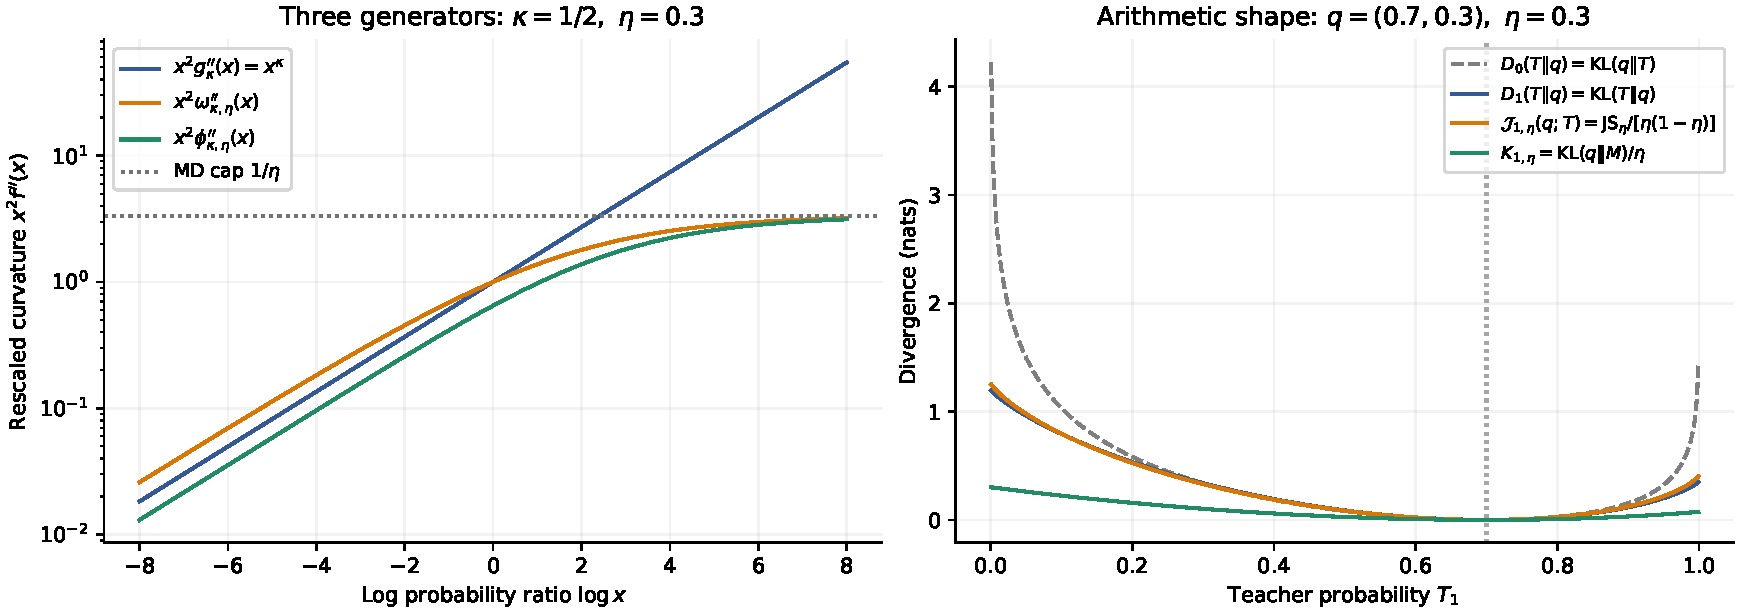
\includegraphics[width=\textwidth]{../../results/power-divergence-relations/families-and-curvature.pdf}
 \caption{三种散度的解析函数比较。左图在 $\kappa=1/2,\eta=0.3$ 时比较乘以 $x^2$ 的生成函数曲率；MD 曲率被 $1/\eta$ 统一控制，中心曲率更小。右图固定 $q=(0.7,0.3)$、$\eta=0.3$，让教师 $T=(T_1,1-T_1)$ 变化；算术形状的重心散度、精确 MD 目标和教师中心分别是 forward KL、归一化 JS 和对混合分布的 reverse KL。所有曲线直接计算公式，不来自训练或模型实验。}
 \label{fig:power-divergence-curvature}
\end{figure}

图的生成入口为 \path{experiments/plotting/plot_power_divergence_relations.py}；参数与公式范围保存在 \path{results/power-divergence-relations/figure.json}。

\begin{corollary}[精确外层的教师监督噪声可求和]
\label{cor:power-md-summable-variance}
固定 $0<\kappa\le1/2$、$0<\eta<1$，采用每步精确幂均值目标的外层 $q_{n+1}=m_{\kappa,\eta}(q_n,T)$。令
\begin{equation}
 V_n=\Var_{q_n}\!\left[A_{\kappa,\eta}(T/q_n)+K_{\kappa,\eta}(q_n,T)\right],
 \qquad C_0=\KL(T\Vert q_0).
\end{equation}
则对 $N\ge1$，
\begin{align}
 V_N&\le\frac{C_0}{\kappa(1-\kappa)(1-\eta)^2\eta N},\\
 \sum_{n=1}^N V_n&\le\frac{C_0}{\kappa(1-\kappa)(1-\eta)^2\eta}.
 \label{eq:power-md-summable-variance}
\end{align}
若各 outer 起点的 score 统一满足 $\|\psi_n(a)\|\le S$，则中心化 teacher score 单样本梯度的协方差 trace 也分别不超过右侧乘以 $S^2$。
\end{corollary}

\begin{proof}
第~\ref{thm:center-advantage-variance}~定理给出 $V_n\le K_n/[\kappa(1-\kappa)(1-\eta)^2]$；第~\ref{thm:power-md-center-comparison}~定理给出 $K_n\le\mathcal J(q_n;T)$。将两者与最后迭代界相乘，得到第一式。三点进展的望远镜求和给出 $\eta\sum_{n=1}^N\mathcal J(q_n;T)\le C_0$，代入得到第二式。梯度方差不超过其二阶矩，且 $\E_{q_n}\|\psi_n B_n\|^2\le S^2V_n$，得到带 score 的结论。
\end{proof}

可求和性针对同一固定 prefix、精确刷新分布和未标准化的教师监督。它并不比较每个输入上不同 $\kappa$ 的实际方差，也不覆盖任意神经网络 inner 残差或不断改变的 prefix 访问测度。该推论把“鲁棒散度有界”“新目标的精确 MD 下降”和“误差相关方差界”连接为一条完整论证；无需先做大模型扫描来确定这些条件性质。
